\newpage
\section{590. N叉树的后序遍历}
\label{leetcode:590}

\subsection{题目}

给定一个 N 叉树,返回其节点值的后序遍历。

例如,给定一个 3叉树 :

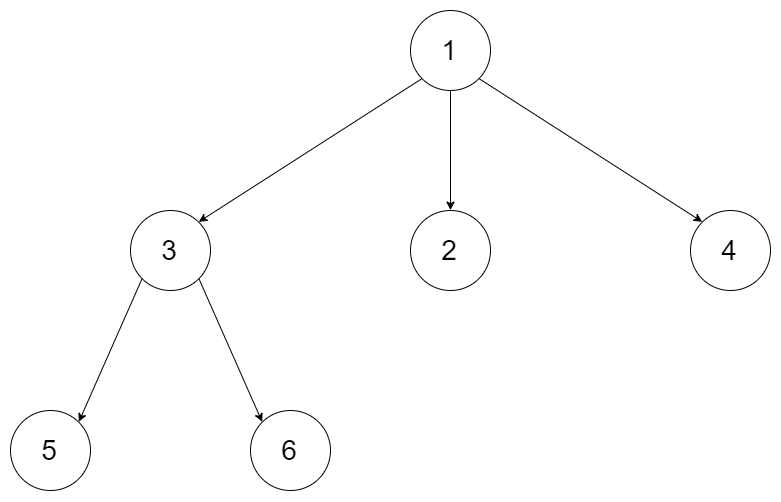
\includegraphics[width=70mm,height=50mm]{images/leetcode/leetcode_429_narytreeexample.png}

返回其后序遍历: [5,6,3,2,4,1]。

说明: 递归法很简单,你可以使用迭代法完成此题吗?

\subsection{参考题解}

\begin{verbatim}
/**
 * // Definition for a Node.
 * function Node(val,children) {
 *    this.val = val;
 *    this.children = children;
 * };
 */
/**
 * @param {Node} root
 * @return {number[]}
 */
var postorder = function(root) {
  let result = [];
  recursion(root, result);
  return result;
};

function recursion(root, result) {
  if (root === null) { return; }
  for (let i = 0; i < root.children.length; i += 1) {
    recursion(root.children[i], result);
  }
  result.push(root.val);
}
\end{verbatim}